\documentclass{article}
\usepackage[utf8]{inputenc}
\usepackage{graphicx}
\usepackage{amsmath}
\title{Regneoppgaver 3}
\author{Mads Balto}
\date{February 2022}
%self defined commands
%%english
\newcommand{\ex}[1]{\section*{exercice #1}}
\newcommand{\subex}[1]{\subsection*{#1)}}
%%norwegian
\newcommand{\opg}[1]{\section*{Oppgave #1}}
\newcommand{\subopg}[1]{\subsection*{#1)}}




\begin{document}


\maketitle
\opg{1}
Vi har at $f_1=1485$KHz, og at $\Delta f \geq 9$KHz. Dette medfører at $f_2 \geq 1494$KHz. Vi bruker at $Q = \frac{f}{\Delta f}$, og finner en Q-faktor på 165 eller lavere.
\opg{2}
\subopg{a}
Vi bruker to arrays for k, en der k vokser lineært $k_lin$, og en som vokser logaritmisk $k_log$. massen er også en array, og regnes ut som produktet av massetetthetsarrayen og volumarrayen $(m = \rho V)$ der, bredden og tykkelsen
forandrer seg lineært, og ganges med lengden $\text{dl}$. dette ganges så med massetetthetsarrayen $\rho$ som også forandrer seg lineært. ved massearrayen konstruert så evaluerer vi vinkelfrekvensen $\omega = \sqrt{\frac{k}{m}}$. til
slutt regner vi ut frekvensen $f=\frac{\omega}{2\pi}$. Bruker dette utrykket til å sammenligne frekvensene $f_{\text{lin}}$ og $f_{}\text{log}}$.
\begin{figure}
    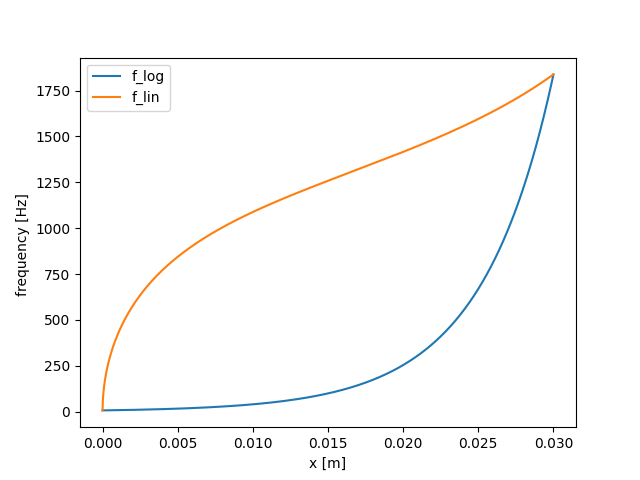
\includegraphics[scale=0.4]{frequency.png}
    \caption{$f_{\text{log}}$ og $f_{\text{lin}}$ som funksjoner av posisjon}
\end{figure}
Vi merker stor forskjell basert på om vi velger lineær forandring, eller logaritmisk forandring for k.
\subopg{b}
Tar i bruk formelen for amplituderesonsans:
\begin{align*}
    A = \frac{F/m}{\sqrt{()\omega_0^2 - \omega_f^2)^2 + (b\omega_f/m)^2}}
\end{align*}
der $\omega_0^2 = \frac{k}{m}$, $F=1$N, $\omega_f=2\pi f$, og $b$ bestemmes. $b$ bestemmes slik at toppene for de forskjellige frekvensene kan skilles, der amplituderesponsen plottes som funksjon av posisjon.
\begin{figure}[h!]
    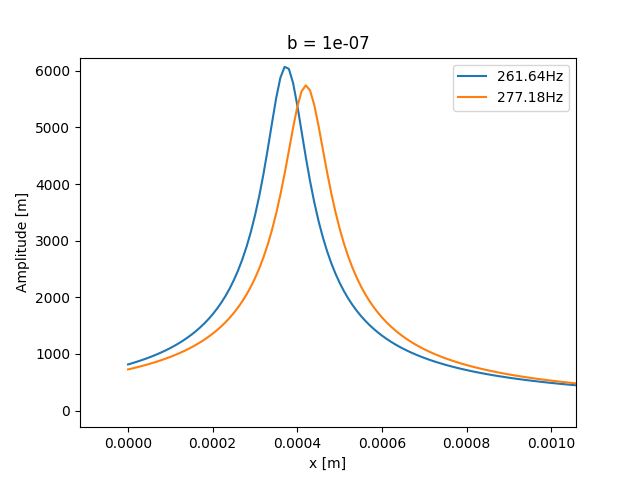
\includegraphics[scale=.5]{b_2_fig_1.png}
    \caption{Amplituderesponsen som funksjon av tid. Her er $b = 10^{-7}$}
\end{figure} 
\begin{figure*}[h!]
    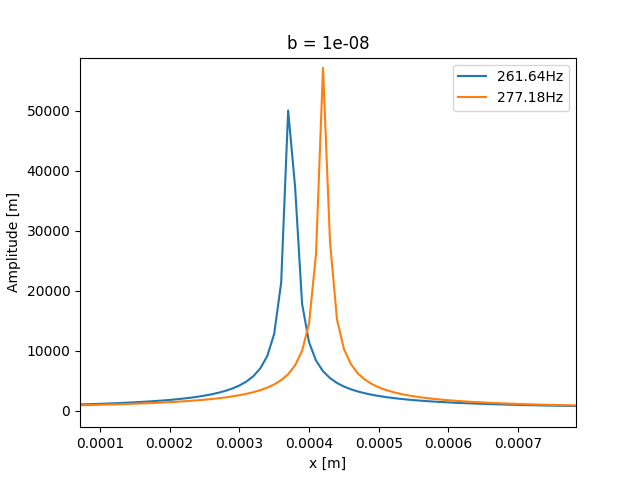
\includegraphics[scale=.5]{b_2_fig_2.png}
    \caption{Amplituderesponsen som funksjon av tid. Her er $b=10^{-8}$}
\end{figure*}
I figurene ser vi at toppene går fra å være for det meste overlappende, til å være ganske så separat i overgangen fra $b=10^{-7}$ til $10^{-8}$.
\subopg{c}
Vi bruker at $Q=\frac{m\omega_0}{b}$ og ved valg av elementene i arraysa med indeks tilsvarende der frekvensen til f1 er størst, så finner vi at kvalitetsfaktoren $Q\approx 75.45$.
\subopg{d}
Vi bruker at $\Delta t = \frac{Q}{\omega_0}$ for å beregne hvor lenge øret vibrerer. Igjen bruker tilsvarende indeks der f_1 arrayen er størst, Får da at tiden det tar for vibrasjonen å stoppe er$\Delta t = 0.04$ms


\opg{3}
\subopg{a}
Vi har at
\begin{align*}
    &L \ddot{Q}+ \dot{Q}R + \frac{Q}{C} = V_0\cos(\omega t)\\
    &\Rightarrow L\ddot{Q} = V_0\cos(\omega t)  - R\dot{Q} -\frac{Q}{C}\\
\end{align*}
Dette er analogt til mekaniske systemer:
\begin{align*}
    F\cos (\omega_Ft) - kz -b \dot{z} = m\ddot{z}
\end{align*}
Da faller det ut at $m=L$, $k=\frac{1}{C}$, og $b=R$, og $F=V_0$. Dette medfører at:
\begin{align*}
    &\omega_0^2 =\frac{k}{m} = \frac{1}{LC}\\
    &\omega_F = \sqrt{w_0^2 - \frac{b^2}{2m^2}}\\
    &= \sqrt{\frac{1}{LC} - \frac{R^2}{2L^2}}\\
    &\omega_0^2 - \omega_F^2 =\frac{R^2}{2L^2}\\
    & b\omega_F = (\sqrt{\frac{1}{LC} - \frac{R^2}{2L^2}})R/L
\end{align*}
Regner ut faseskift mellom påtrykt spenning  og ladning på kondensatoren:
\begin{align*}
    \cot \phi  &= \frac{\omega_0^2 - \omega_F^2}{\omega_Fb/m}
    = \frac{\frac{R^2}{2L^2}}{(\sqrt{\frac{1}{LC} - \frac{R^2}{2L^2}})R/L}\\
    &= \frac{R}{2L(\sqrt{\frac{1}{LC} - \frac{R^2}{2L^2}}}
\end{align*}
Regner ut amplituden for ladningsoscilasjonene:
\begin{align*}
    A &= \frac{F/m}{\sqrt{(\omega_0^2 - \omega_F^2)^2 + (b\omega_F/m)^2}}\\
    &= \frac{V_0/L}{\sqrt{(\frac{R^2}{2L^2})^2 - (\sqrt{\frac{1}{LC} - \frac{R^2}{2L^2}})R/L)^2}}\\
    &= \frac{V_0/L}{\sqrt{\frac{R^4}{4L^4} -  (\frac{1}{LC} - \frac{R^2}{2L^2})R^2/L^2}}\\
    &= \frac{V_0/L}{\sqrt{\frac{R^4}{4L^4} -  \frac{R^2}{L^3C} + \frac{R^4}{2L^4}}}\\
    &=  \frac{V_0/L}{\sqrt{(\frac{R^2}{L^2})\frac{3R^2}{4L^2} -  \frac{1}{LC} }}\\
    &=\frac{V_0}{R\sqrt{\frac{3R^2}{4L^2} -  \frac{1}{LC}}}
\end{align*}
Regner ut Q verdi:
\begin{align*}
    Q = \sqrt{\frac{mk}{b}}=\sqrt{\frac{L}{R^2c}}
\end{align*}
Regner ut faseresonansfrekvensen:
\begin{align*}
    f_{\text{ph.res}.} = \frac{1}{2\pi}\omega_0 = \frac{1}{2\pi}\sqrt{\frac{1}{LC}}
\end{align*}
regner ut  ampltituderesonans-frekvensen:
\begin{align*}
    f_{\text{amp.res}} &= \frac{1}{2\pi}\omega_F = \frac{1}{2\pi}\sqrt{\frac{1}{LC} - \frac{R^2}{2L^2}}
\end{align*}

\subopg{b}
vi har at $Q=\sqrt{\frac{L}{R^2C}}$. Vi setter inn for $R=1$\Omega, $L=25\text{\mu}$H, og $C=100$nF.
\begin{align*}
    Q = \sqrt{\frac{25\cdot10^{-6}}{1^2\cdot 10^2 10^{-9}}}
    =\sqrt{250}
    =5\sqrt{2}\sqrt{5}\approx 15.811
\end{align*} 
\subopg{c}
vi vet at faseresonans er når $\omega_f = omega_0$. i for Faseresonansen så er altså $\cot\phi = 0$. Dette medfører at $\phi=\frac{\pi}{2}$. Vi vet at $Q = A\cos(\omega_F t)$, og da er strømmen 
$I=\frac{dq}{dt}= -A\omega_F \sin(\omega_Ft)=A\omega_F \cos(\omega_F- \frac{\pi}{2})$. I faseresonans så blir dermed forskjellen i fasevinkel 0.
\end{document}